\section{Das Projekt}
\subsection*{Die Aufgabe}



\begin{frame}{Orchestrierung von Webservices}
	
\begin{center}

\includegraphics[width=\textheight]{Bilder/titel_einfuehrung_logos.png} 
\end{center}

\end{frame}

\begin{frame}{Die Problemstellung}
\begin{itemize}[<+->]
	\item \textbf{Datenmigration:} (Kontakte von SAP zu Google)
	\pause
	\item \textbf{Strategie:} (nicht einfach kopieren $\rightarrow$ Karteileichen)
		\begin{itemize}[<+->]
			\item Kontakte nur bei Bedarf übertragen!
			\pause
			\item zunächst bei Google anfragen
			\item erst dann Migration von SAP
			\item sonst manuelle Eingabe
		\end{itemize}
	\pause
	\item \textbf{erste Überlegungen:}
		\begin{itemize}[<+->]
			\item drei Teile: Google, SAP, SIBs
			\item GUI Elemente für Dateingabe
		\end{itemize}
\end{itemize}
\end{frame}


\begin{frame}{Projekt-Komponenten}
	
\begin{center}
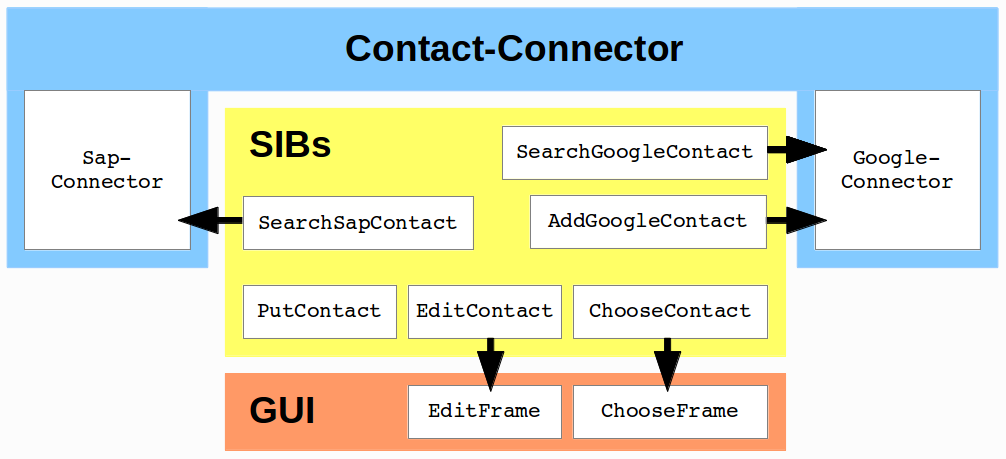
\includegraphics[width=\textheight]{Bilder/projekt_aufbau.png} 
\end{center}

\end{frame}


\begin{frame}{Eingesetzte Tools}
\begin{itemize}[<+->]
	\pause
	\item \textbf{klar:} automatisierte Tests (JUnit), Versionsverwaltung (git)
	\pause
	\item \textbf{Apache Maven:} (Build-Management-Tool)
		\begin{itemize}[<+->]
			\pause
			\item unterstützt Software-Lebenszyklus $\rightarrow$ automatische Ausführung der Tests
			\item einfaches Einbinden von Abhängigkeiten (externe Pakete)
			\item verpackt alle Komponenten zu einer JAR-Datei $\rightarrow$ jABC-Projekt
		\end{itemize}
\end{itemize}
\end{frame}











